\documentclass{article}
\usepackage[utf8]{inputenc}
\usepackage{amsmath}
\usepackage{amssymb}
\usepackage[table]{xcolor}
\usepackage{tikz}
\DeclareRobustCommand{\DirectNESS}{(\tikz[baseline=-\the\dimexpr\fontdimen22\textfont2\relax,inner sep=0pt] \draw[dash pattern={on 4.5pt off 4.5pt}](0,0) -- (5mm,0);)}
\DeclareRobustCommand{\NESS}{(\tikz[baseline=-\the\dimexpr\fontdimen22\textfont2\relax,inner sep=0pt] \draw[dash pattern={on 0.84pt off 2.51pt}](0,0) -- (5mm,0);)}
\DeclareRobustCommand{\actual}{(\tikz[baseline=-\the\dimexpr\fontdimen22\textfont2\relax,inner sep=0pt] \draw[line width=0.75](0,0) -- (5mm,0);)}

\begin{document}

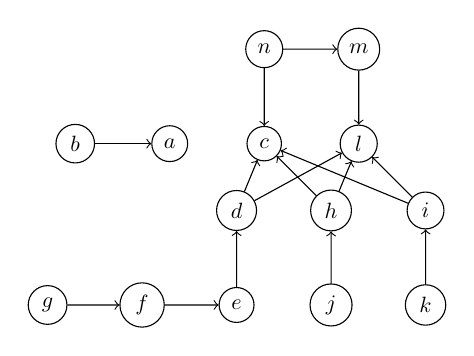
\begin{tikzpicture}[scale=0.8,transform shape, node distance={15mm}, main/.style = {draw, circle}]
            
                \node[main] (1) {$a$}; 
                \node[main] (2) [left of=1] {$b$};
                \node[main] (3) [right of=1] {$c$};
                \node[main] (4) [right of=3] {$l$};
                \node[main] (5) [below right of=3] {$h$};
                \node[main] (6) [left of=5] {$d$};
                \node[main] (7) [right of=5] {$i$};
                \node[main] (8) [above of=3] {$n$};
                \node[main] (9) [above of=4] {$m$};
                \node[main] (10) [below of=6] {$e$};
                \node[main] (11) [below of=5] {$j$};
                \node[main] (12) [below of=7] {$k$};
                \node[main] (13) [left of=10] {$f$};
                \node[main] (14) [left of=13] {$g$};
                
                
                
                \draw[->] (2) -- (1);
                \draw[->] (5) -- (3);
                \draw[->] (6) -- (3);
                \draw[->] (7) -- (3);
                \draw[->] (8) -- (3);
                \draw[->] (5) -- (4);
                \draw[->] (6) -- (4);
                \draw[->] (7) -- (4);
                \draw[->] (9) -- (4);
                \draw[->] (10) -- (6);
                \draw[->] (13) -- (10);
                \draw[->] (14) -- (13);
                \draw[->] (11) -- (5);
                \draw[->] (12) -- (7);
                \draw[->] (8) -- (9);
                
            \end{tikzpicture}

\end{document}